% ||||||||||||||||||||||||||||||||||||||||||||||
% Capitulo de Revisão Bibliográfica
% ||||||||||||||||||||||||||||||||||||||||||||||

\chapter{Revisão Bibliográfica}

Fazer:
\begin{itemize}
    \item Conceito básico de máquinas rotativas
    \item Conceito de Motor Elétricos
    \item Falar de motores elétricos CC e, por último, sobre Indução, fazendo o link com a próxima etapa
\end{itemize}

%++++++++++++++++++++++++++++++++++++++++++++++++++++++++++++++++
% 
%++++++++++++++++++++++++++++++++++++++++++++++++++++++++++++++++

\section{Motores Elétricos de Indução}\label{sec:}

Fazer:
\begin{itemize}
    \item conceitos gerais usando Fitzgerald
    \item Rotor
    \item Estator
    \item Buscar algo sobre corrente elétrica ou complementar em relação ao circuito equivalente
\end{itemize}

\begin{figure}[H]
    \caption{Motor elétrico de indução tipo gaiola de esquilo.}
    \begin{center}
        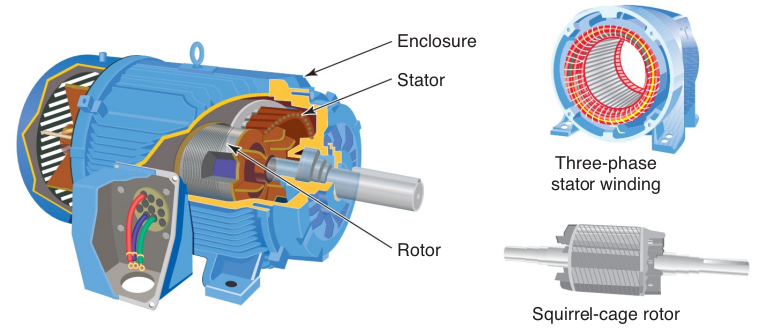
\includegraphics[scale=.5]{referencial/img/ind_motor_petruzella_p115.png}
    \end{center}
    \fonte{\citeonline{Petruzella1911}.} 
    \label{fig:}
\end{figure}



\begin{figure}[H]
    \caption{Circuito equivalente monofásico de um motor indutivo polifásico.}
    \begin{center}
        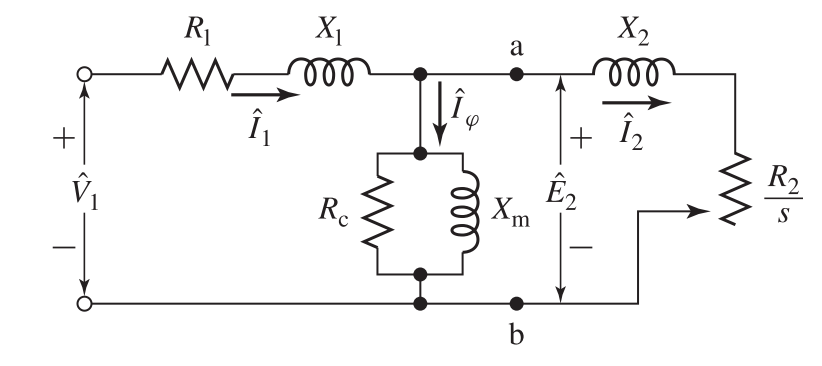
\includegraphics[scale=.35]{referencial/img/circuit_fitzgerald_p354.png}
    \end{center}
    \fonte{\citeonline{Umans2003}.} 
    \label{fig:}
\end{figure}


%----------------------------------------------------------------
% 
%----------------------------------------------------------------

\section{Falhas em Motores Elétricos de Indução}\label{sec:}

Fazer:
\begin{itemize}
    \item Conceitos básicos e a importância das falhas
    \item Listar as principais falhas e lincar com os efeitos
    \item explicar a imagem sobre todos os tipos de falhas e elencar as mais comuns via refêrencia
    \item após a etapa acima, apresentar os principais problemas de acordo com as imagens
\end{itemize}

\begin{figure}[H]
    \caption{Variação da carga para distinção da causa do efeito observado.}
    \begin{center}
        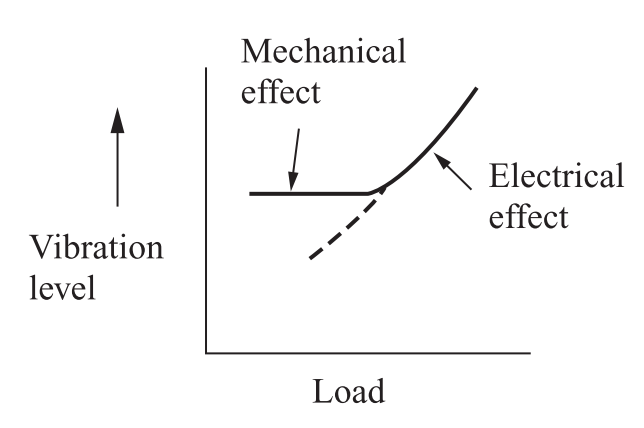
\includegraphics[scale=.45]{referencial/img/fault_effect_randall_p54.png}
    \end{center}
    \fonte{\citeonline{Wu2013}.} 
    \label{fig:}
\end{figure}


\begin{figure}[H]
    \caption{Árvo dos principais tipos de falhas em motores elétricos.}
    \begin{center}
        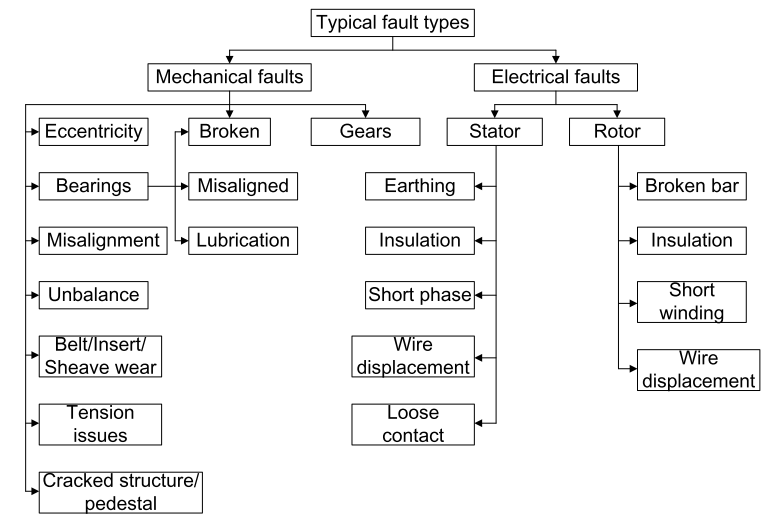
\includegraphics[scale=.5]{referencial/img/faults_rilski_p77.png}
    \end{center}
    \fonte{\citeonline{Gorbounov2018}.} 
    \label{fig:}
\end{figure}


\begin{figure}[H]
    \caption{Ilustração com as frequências associadas as falhas em rotores ou estatores de motores elétricos.}
    \begin{center}
        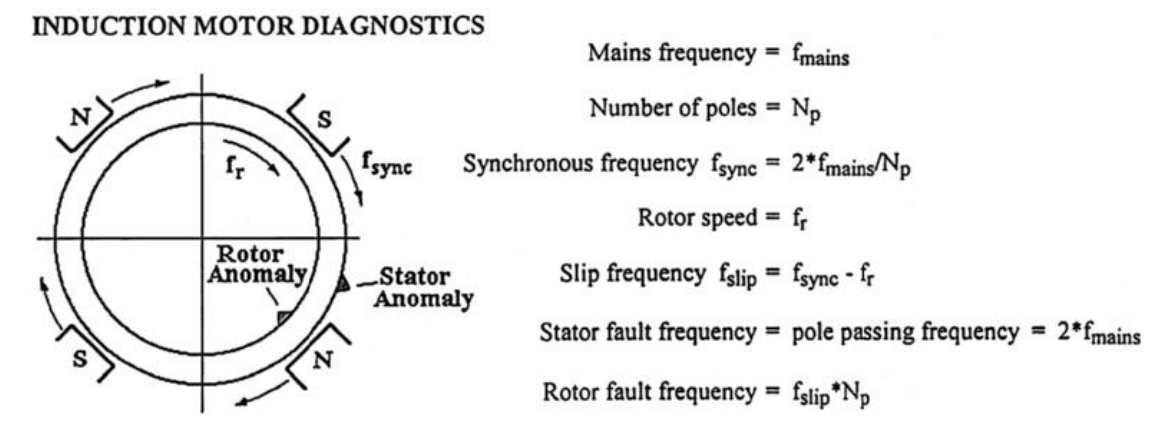
\includegraphics[scale=.35]{referencial/img/fault_freq_randall_p55.png}
    \end{center}
    \fonte{\citeonline{Wu2013}.} 
    \label{fig:}
\end{figure}


\begin{figure}[H]
    \caption{Ilustração com os tipos de desalinhamento.}
    \begin{center}
        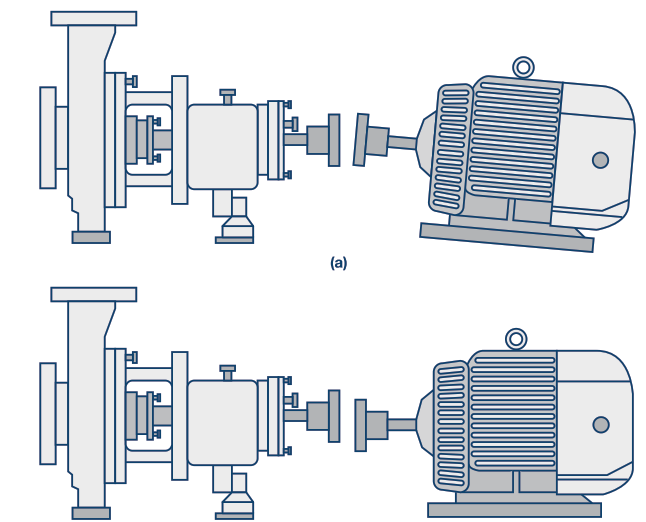
\includegraphics[scale=.45]{referencial/img/misadraw_analog_p2.png}
    \end{center}
    \fonte{\citeonline{Sopcik2019}.} 
    \label{fig:}
\end{figure}


\begin{figure}[H]
    \caption{Imagens de rolamentos no topo, e falhas na parte de baixo.}
    \begin{center}
        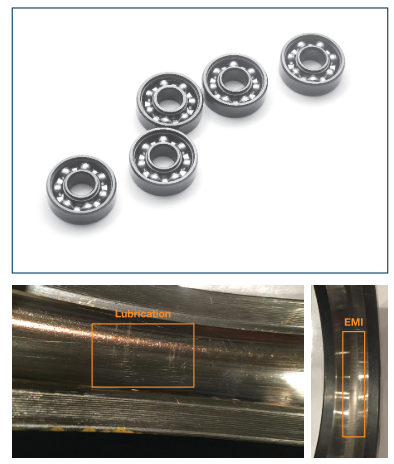
\includegraphics[scale=.5]{referencial/img/bearing_analog_p3.png}
    \end{center}
    \fonte{\citeonline{Sopcik2019}.} 
    \label{fig:}
\end{figure}

%++++++++++++++++++++++++++++++++++++++++++++++++++++++++++++++++
% 
%++++++++++++++++++++++++++++++++++++++++++++++++++++++++++++++++

\section{Análise de Vibração}\label{sec:}

Fazer:
\begin{itemize}
    \item breve esclarecimento entre os sinais amostrados e o espectro
    \item explicação sobre a amostragem nesses casos
\end{itemize}

\begin{figure}[H]
    \caption{Valores máximos de velocidade RMS para cada porte de máquina indicados pela norma ISO 10816-1.}
    \begin{center}
        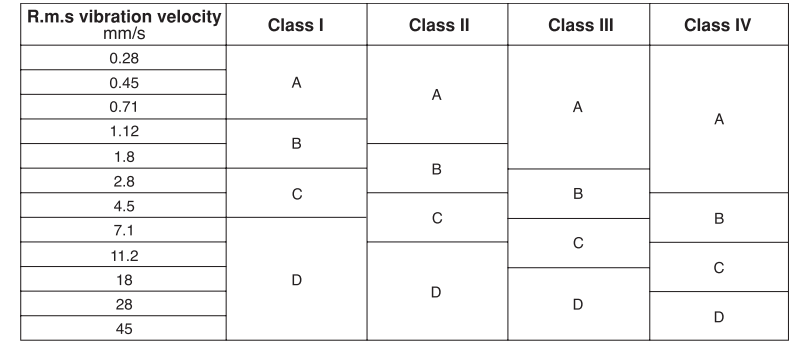
\includegraphics[scale=.5]{referencial/img/iso10816-1_randall_p146.png}
    \end{center}
    \fonte{\citeonline{Wu2013}.} 
    \label{fig:}
\end{figure}

\begin{figure}[H]
    \caption{Indicação espectral de desalinhamento.}
    \begin{center}
        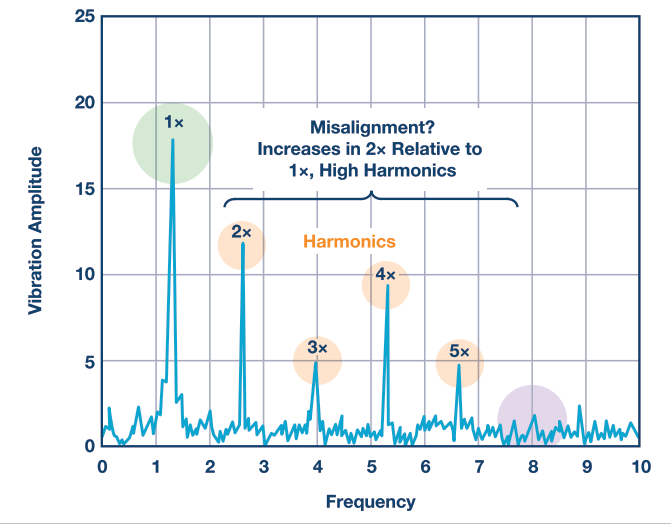
\includegraphics[scale=.4]{referencial/img/misa_analog_p2.png}
    \end{center}
    \fonte{\citeonline{Sopcik2019}.} 
    \label{fig:}
\end{figure}

\begin{figure}[H]
    \caption{Indicação espectral de desbalanceamento.}
    \begin{center}
        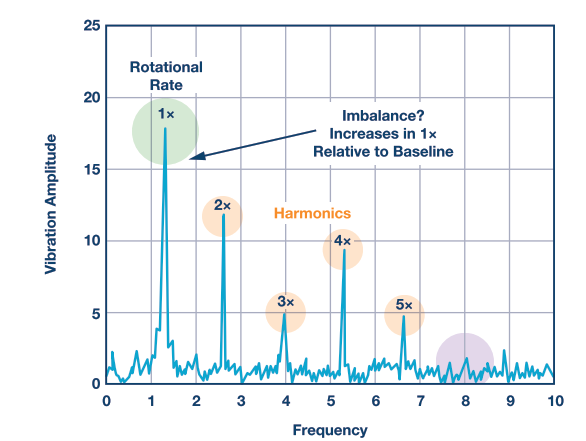
\includegraphics[scale=.5]{referencial/img/imbalance_analog_p2.png}
    \end{center}
    \fonte{\citeonline{Sopcik2019}.} 
    \label{fig:}
\end{figure}


%++++++++++++++++++++++++++++++++++++++++++++++++++++++++++++++++
% 
%++++++++++++++++++++++++++++++++++++++++++++++++++++++++++++++++

\section{Sistemas de Detecção de Falhas}\label{sec:}

\begin{figure}[H]
    \caption{Árvo de métodos de monitoramento de falhas em motores elétricos.}
    \begin{center}
        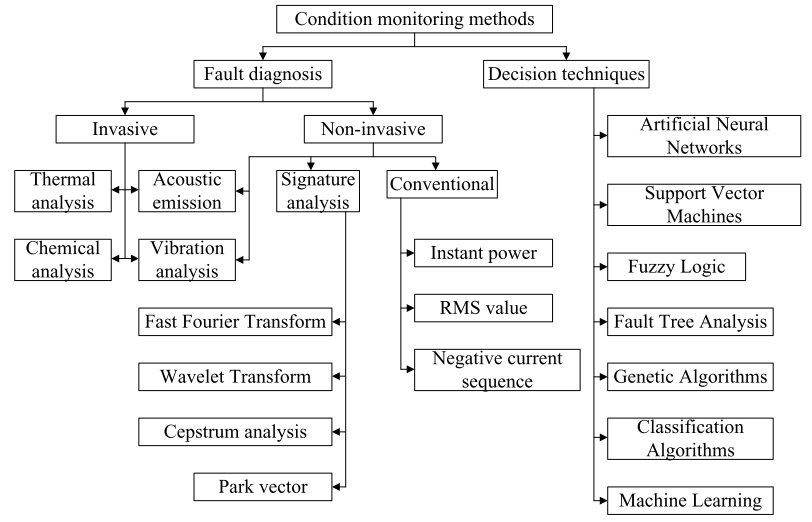
\includegraphics[scale=.5]{referencial/img/monitoring_methods_rilski_p78.png}
    \end{center}
    \fonte{\citeonline{Gorbounov2018}.} 
    \label{fig:}
\end{figure}


%++++++++++++++++++++++++++++++++++++++++++++++++++++++++++++++++
% 
%++++++++++++++++++++++++++++++++++++++++++++++++++++++++++++++++

\subsection{Análise de Corrente Elétrica }\label{sec:}


\begin{figure}[H]
    \caption{Proposta de sistema de diagnóstico utilizando a corrente do estator.}
    \begin{center}
        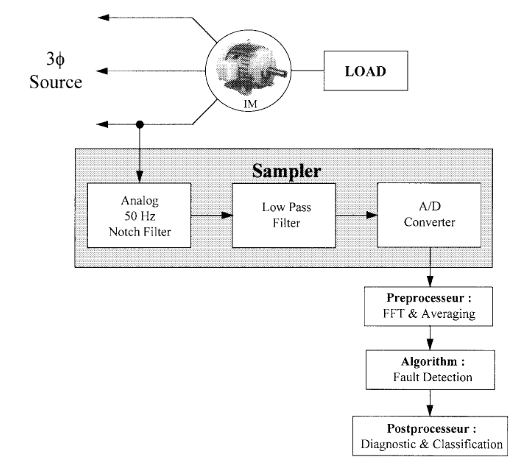
\includegraphics[scale=.5]{referencial/img/current_benbouzid_p3.png}
    \end{center}
    \fonte{\citeonline{El1999}.} 
    \label{fig:}
\end{figure}

%++++++++++++++++++++++++++++++++++++++++++++++++++++++++++++++++
% 
%++++++++++++++++++++++++++++++++++++++++++++++++++++++++++++++++

\section{Técnicas Modernas de Processamento de Sinais}\label{sec:}



%----------------------------------------------------------------
% 
%----------------------------------------------------------------

\subsection{RNA}

\begin{figure}[H]
    \caption{Rede neural convolucional.}
    \begin{center}
        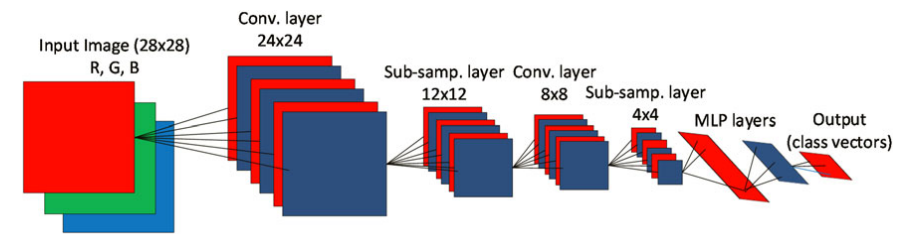
\includegraphics[scale=.4]{referencial/img/cnn_image_ince_p5.png}
    \end{center}
    \fonte{\citeonline{Ince2016}.} 
    \label{fig:}
\end{figure}


%----------------------------------------------------------------
% 
%----------------------------------------------------------------

\subsection{ICA}

\begin{figure}[H]
    \caption{Fluxograma do algoritmo fastICA.}
    \begin{center}
        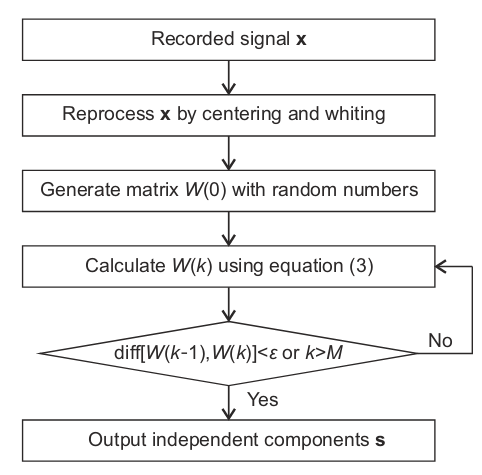
\includegraphics[scale=.5]{referencial/img/fatica_fang_p3.png}
    \end{center}
    \fonte{Duan2017.} 
    \label{fig:}
\end{figure}


%----------------------------------------------------------------
% 
%----------------------------------------------------------------

\subsection{T-SNE}

\begin{figure}[H]
    \caption{Algoritmo simplificado da técnica t-SNE.}
    \begin{center}
        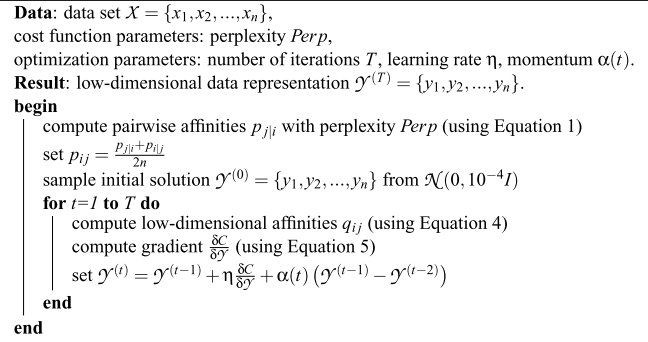
\includegraphics[scale=.45]{referencial/img/t-sne_algorithm_maaten_p9.png}
    \end{center}
    \fonte{\citeonline{VanDerMaaten2008}.} 
    \label{fig:}
\end{figure}

%----------------------------------------------------------------
% 
%----------------------------------------------------------------

\subsection{K-Means}

\begin{figure}[H]
    \caption{Exemplo de clusterização utilizando K-means.}
    \begin{center}
        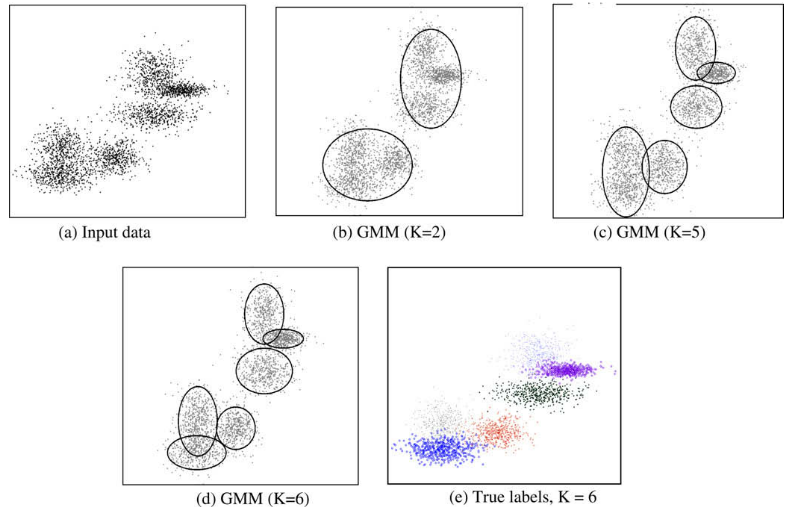
\includegraphics[scale=.5]{referencial/img/k-means_jain_p7.png}
    \end{center}
    \fonte{\citeonline{Jain2010}.} 
    \label{fig:}
\end{figure}


%++++++++++++++++++++++++++++++++++++++++++++++++++++++++++++++++
% 
%++++++++++++++++++++++++++++++++++++++++++++++++++++++++++++++++

\section{Estado da Arte}


%----------------------------------------------------------------
% 
%----------------------------------------------------------------

\subsection{CNN}

\begin{figure}[H]
    \caption{Diagrama de um sistema que utiliza CNN.}
    \begin{center}
        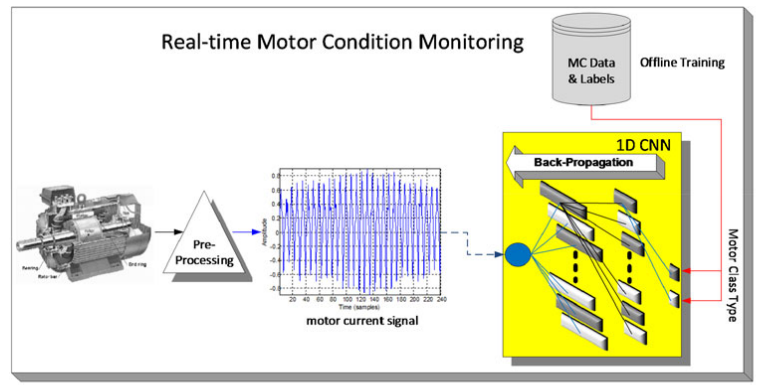
\includegraphics[scale=.45]{referencial/img/cnn_ince_p2.png}
    \end{center}
    \fonte{\citeonline{Ince2016}.} 
    \label{fig:}
\end{figure}


\begin{figure}[H]
    \caption{Diagrama de uma técnica que utiliza classificação de orbitais com CNN.}
    \begin{center}
        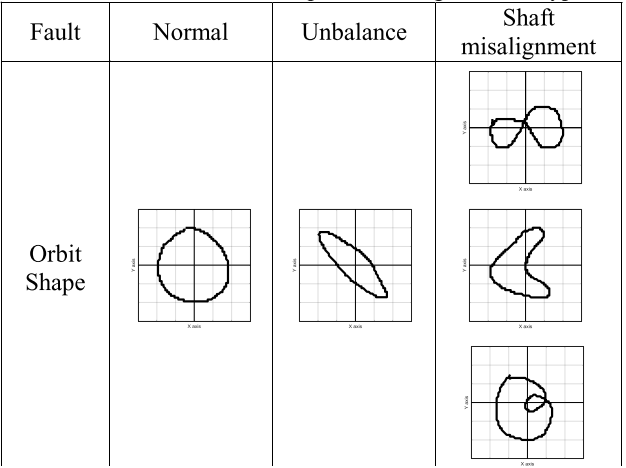
\includegraphics[scale=.45]{referencial/img/orbit_jeong_p3.png}
    \end{center}
    \fonte{\citeonline{Jeong2016}.} 
    \label{fig:}
\end{figure}

\begin{figure}[H]
    \caption{Técnica com Back-programation.}
    \begin{center}
        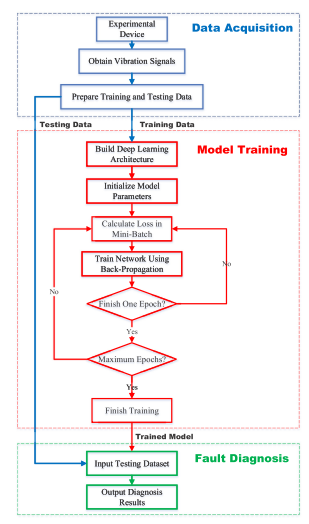
\includegraphics[scale=.65]{referencial/img/back-programation-zhang-p5.png}
    \end{center}
    \fonte{\citeonline{Zhang2018}.} 
    \label{fig:}
\end{figure}


%----------------------------------------------------------------
% 
%----------------------------------------------------------------

\subsection{ICA}

\begin{figure}[H]
    \caption{Fluxograma de uma técnica que utiliza ICA.}
    \begin{center}
        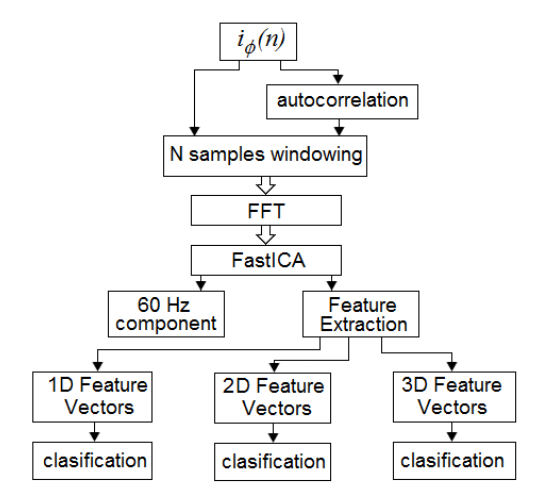
\includegraphics[scale=.5]{referencial/img/ica_bracamonte_p4.png}
    \end{center}
    \fonte{\citeonline{Garcia-Bracamonte2019}.} 
    \label{fig:}
\end{figure}


%----------------------------------------------------------------
% 
%----------------------------------------------------------------

\subsection{WPT (\textit{Wavelet Packet Transform})}

\textbf{VER COM O RODRIGO, PORQUE NÃO EXPLIQUEI O ASSUNTO E NÃO APLIQUEI NOS RESULTADOS}